% arara: clean: {files: [thesis.aux, thesis.idx, thesis.ilg, thesis.ind, thesis.log, thesis.bbl, thesis.bcf, thesis.ist, thesis.blg, thesis.run.xml, thesis.lol, thesis.out, thesis.toc, texput.log]}
% arara: lualatex: { shell : yes , action: batchmode}
% arara: lualatex: { shell : yes , action: batchmode}

\documentclass[a4paper,11pt]{kth-mag}
\DeclareMathSizes{10.95}{12}{9}{7}

% Math and code packages
\usepackage{amsmath}   % all things math
\usepackage{amssymb}   % additional math symbols
\usepackage{xfrac}     % nice fractions in body of text
\usepackage{siunitx}   % typesets numbers with units
\usepackage{mathtools} % extensions for amsmath
\usepackage[section]{minted}    % advanced code examples

% Tables
\usepackage{booktabs} % professionally looking tables
\usepackage{tabulary} % whole page tables

% Caption and split floats
\usepackage{caption}    % customizable captions
\usepackage{subcaption} % nice subfigures and subtables

% Bibliographies
\usepackage[backend=biber]{biblatex} % modern bibliographies
\usepackage{csquotes}

% PDF Metadata
\usepackage{hyperref} % enables PDF hyperlinks

% Fonts, typography and languages
\usepackage{fontspec}     % all things fonts
\defaultfontfeatures{Ligatures=TeX}
\setmainfont{FiraSans-Book.otf}[
  BoldFont = FiraSans-SemiBold.otf,
  ItalicFont = FiraSans-Italic.otf,
  BoldItalicFont = FiraSans-SemiBoldItalic.otf]
\setsansfont{FiraSans-Regular.otf}[Scale=MatchLowercase]
\setmonofont{FiraMono-Regular.otf}[Scale=MatchLowercase]
\usepackage{unicode-math} % use custom fonts for math
\setmathfont{Asana-Math.otf}
\usepackage{microtype}	  % advanced typesetting
\DisableLigatures{family=tt*}
\usepackage[main=english, swedish]{babel} % language-specific conventions

% Graphics
\usepackage{graphicx} % all things graphics
\usepackage{pgfplots} % complex graphs
\usepgfplotslibrary{dateplot}
\usepackage{pgfplotstable}
\pgfplotsset{
  compat=1.11, % avoid running in backwards compatibility mode
  width=\textwidth,
  tick label style = {font=\ttfamily},
  every axis label = {font=\sffamily},
  legend style = {font=\sffamily},
  label style = {font=\sffamily},
  separate axis lines,
  y axis line style={draw opacity=0},
  x axis line style={gray},
  axis x line*=bottom,
  axis y line*=left,
  major tick length=0pt,
  grid=both,
  y grid style={dashed},
  legend pos=north west,
}
\definecolor{set11}{RGB}{228,  26,  28}
\definecolor{set12}{RGB}{ 55, 126, 184}
\definecolor{set13}{RGB}{ 77, 175,  74}
\definecolor{set14}{RGB}{152,  78, 163}
\definecolor{set15}{RGB}{255, 127,   0}
\definecolor{set16}{RGB}{255, 255,  51}
\definecolor{set17}{RGB}{166,  86,  40}
\definecolor{set18}{RGB}{247, 129, 191}
\definecolor{set19}{RGB}{153, 153, 153}

\definecolor{set11_light}{RGB}{251, 180, 174}
\definecolor{set12_light}{RGB}{179, 205, 227}
\definecolor{set13_light}{RGB}{204, 235, 197}
\definecolor{set14_light}{RGB}{222, 203, 228}
\definecolor{set15_light}{RGB}{254, 217, 166}
\definecolor{set16_light}{RGB}{255, 255, 204}
\definecolor{set17_light}{RGB}{229, 216, 189}
\definecolor{set18_light}{RGB}{253, 218, 236}
\definecolor{set19_light}{RGB}{242, 242, 242}

% \definecolor{set11}{cmyk}{.1 ,.9 ,.8 ,.0 }
% \definecolor{set12}{cmyk}{.8 ,.3 ,.0 ,.0 }
% \definecolor{set13}{cmyk}{.7 ,.0 ,.8 ,.0 }
% \definecolor{set14}{cmyk}{.4 ,.65,.0 ,.0 }
% \definecolor{set15}{cmyk}{.0 ,.5 ,1.0,.0 }
% \definecolor{set16}{cmyk}{.0 ,.0 ,.8 ,.0 }
% \definecolor{set17}{cmyk}{.35,.6 ,.8 ,.0 }
% \definecolor{set18}{cmyk}{.0 ,.5 ,.0 ,.0 }
% \definecolor{set19}{cmyk}{.0 ,.0 ,.0 ,.4 }
%
% \definecolor{set11_light}{cmyk}{.0 ,.3 ,.2 ,.0 }
% \definecolor{set12_light}{cmyk}{.3 ,.1 ,.0 ,.0 }
% \definecolor{set13_light}{cmyk}{.2 ,.0 ,.2 ,.0 }
% \definecolor{set14_light}{cmyk}{.12 ,.17,.0 ,.0 }
% \definecolor{set15_light}{cmyk}{.0 ,.15 ,.3,.0 }
% \definecolor{set16_light}{cmyk}{.0 ,.0 ,.2 ,.0 }
% \definecolor{set17_light}{cmyk}{.1,.12 ,.2 ,.0 }
% \definecolor{set18_light}{cmyk}{.0 ,.15 ,.0 ,.0 }
% \definecolor{set19_light}{cmyk}{.0 ,.0 ,.0 ,.05 }

\usepackage{modifications}

\linespread{1.2}

\title{GPU Simulation of Rigid Fibers}

\foreigntitle{GPU simulering av stela fibrer}

\author{Eric Wolter}
\date{January 2015}
\blurb{Master's Thesis at School of Engineering Sciences\\Supervisor: Katarina Gustavsson\\Examiner: Michael Hanke}
\trita{TRITA xxx yyyy-nn}

\begin{document}
\frontmatter
\pagestyle{empty}

\maketitle
\selectlanguage{english}
\begin{abstract}
The major objective of this Master's thesis is to accelerate a serial implementation of a numerical algorithm for the simulation of slender fiber dynamics by using Graphical Processing Units (GPU). We focus on rigid fibers sedimenting due to gravity in a free-space Stokes flow. The ability to simulate a large number of fibers in a reasonable computational time on a high-performance parallel platform opens exciting new research opportunities.

The previous serial implementation is rewritten for parallel execution. The algorithm is implemented in single precision using the Compute Unified Device Architecture (CUDA) on NVIDIA GPUs. In addition, we develop an OpenMP version of the parallel implementation to run on multi-core CPUs. Using both implementations, we perform a number of benchmarks to determine the fastest variant of the algorithm. We observe a speedup of $20×$ to $40×$ on the NVIDIA GTX 970 compared to an Intel Core i7 4770. The GPU implementation can simulate up to $2000$ fibers on a desktop computer and it takes only in the order of $8$ seconds to advance one time step.

Furthermore, we have performed a number of simulations of known experiments for sedimenting fibers to validate the algorithm and to explore the numerical precision of the results. The results show an excellent agreement with results from prior experiments in the field.
\end{abstract}

\clearpage


\begin{foreignabstract}{swedish}
Lorem ipsum dolor sit amet, consectetuer adipiscing elit. Mauris
purus. Fusce tempor. Nulla facilisi. Sed at turpis. Phasellus eu
ipsum. Nam porttitor laoreet nulla. Phasellus massa massa, auctor
rutrum, vehicula ut, porttitor a, massa. Pellentesque fringilla. Duis
nibh risus, venenatis ac, tempor sed, vestibulum at, tellus. Class
aptent taciti sociosqu ad litora torquent per conubia nostra, per
inceptos hymenaeos.
\end{foreignabstract}

\clearpage

\tableofcontents*

\clearpage

\listoflistings

\mainmatter
\pagestyle{newchap}

\chapter{Introduction}

\chapter{Theoretical Foundation}
\label{cha:theoretical_foundation}
The introduction discussed different applications of rigid fiber simulations. It especially stressed the importance of being able to simulate as many fibers as possible to generate the various patterns found in real world experiments.

In this chapter we will present the theoretical foundation of the physics the simulations are based on. This is required to be able to understand the numerical method used throughout the rest of the thesis. However, the method is only presented in a reduced summary for more details please refer to \cite{}.

We will begin by introducing the Stokes flow and its fundamental solutions as they apply to suspended fibers. Afterwards we will focus on the implications this has and how the flow properties can be calulated for the special case of straight and rigid fibers.

\section{Stokes flow}

The aim of the presented simulation is to model the behaviour of objects immersed in a fluid. We restrict ourselves to rigid bodies, which are slowly sedimenting in a viscous fluid due to gravity. The velocity of these rigid objects is only dependent on their orientation and the resulting drag. The interaction between multiple objects is only modeled through the surrounding fluid as collision are not modelled.

\begin{equation}
  \label{eq:naviar_stokes_equations}
  \begin{aligned}
    \rho(\frac{\delta \mathbf{u}}{\delta t} + (\mathbf{u} \cdot \nabla)\mathbf{u}) &= -\nabla p + \mu\nabla^2\mathbf{u} + \mathbf{f}
    \nabla \cdot \mathbf{u} &= 0
  \end{aligned}
\end{equation}

The Naviar-Stokes equations describe the motion of fluids and allow to model the flow around an object. Using and solving theses equations is however quite challenging due to their time depedence and non-linearity. Fortunately we can make a number of simplification due to the restriction we placed on our model. Our model is characterized by three properties.

\begin{enumerate}
  \item{\textit{Newtonian fluid} — The viscosity $\mu$ of the fluid does not depend on the stress.}
  \item{\textit{Incompressible flow} — The density of the fluid does not change.}
  \item{\textit{Low Reynolds number $Re = \frac{\rho U L}{\mu} \ll 1$} — The fluid velocities are very slow and/or the viscosity is very large.}
\end{enumerate}

Given these constraints and especially the very low Reynolds number due to slowly sedimenting objects in a viscous fluid the Naviar-Stokes equations can be linearized to arrive at the Stokes Equations

\begin{equation}
\label{eq:stokes_equations}
\begin{aligned}
    \nabla p - \mu \Delta \mathbf{u} &= \mathbf{f} \quad &\text{in} \quad \Omega \text{,}\\
    \nabla \cdot \mathbf{u} &= 0 \quad &\text{in} \quad \Omega \text{,}
\end{aligned}
\end{equation}

where $\mathbf{u}(\mathbf{x})$ denotes the velocity field, $p(\mathbf{x})$ the pressure field and $\mathbf{f}(\mathbf{x})$ the force acting on the fluid at the location $\mathbf{x} = (x,y,z) \in \mathbb{R}^3$.
The constant $\mu$ is the viscosity of the fluid.

\section{Stokeslet}

The Stokes Equations are linear in both the velocity and pressure, which allow them to be solved using a number of different methods for linear differential equations. Additionally, the equations are time independent and time depedence is only reintroduced due to the motion of the immersed objects and the boundary conditions. Thus given the boundary conditions the structure of the flow can be calculated.

For our model we define two boundary conditions. First we force the fluid velocity at the boundary of the object to be equal to the velocity of the object itself. These no-slip conditions on the surface of the objects are defined as
\begin{equation}
  \label{eq:boundary_condition_surface}
  \mathbf{u} = \mathbf{u}_\Gamma  \quad \text{on} \quad  \Gamma \text{,}
\end{equation}
where $\Gamma$ denotes the union of all body surfaces and $\mathbf{u}_\Gamma$ the corresponding surface velocity, thus constraining the fluid to have zero velocity relative to the surface boundary.

The second boundary condition models the fact that the fluid velocity far from the object is not affected by its presence. This is modeled by the velocity field should be equal to a background velocity $\mathbf{U}_0(\mathbf{x})$ at infinity
\begin{equation}
  \label{eq:boundary_condition_background}
  \mathbf{u} \rightarrow \mathbf{U}_0 \quad \text{as} \quad ||\mathbf{u}|| \rightarrow \infty \text{,}
\end{equation}
enforcing that the velocity field $\mathbf{u}$ should be equal to a background velocity $\mathbf{U}_0(\mathbf{x})$ at infinity. In our simulations this background velocity is always set to $0$.

By taking advantage of the linearity of the Stokes equations and these boundary conditions so-called fundamental solution can be found. For this the force term in Stokes equation~\eqref{eq:stokes_equations} is replaced by a point force acting at the origin $\mathbf{x}_0$
\begin{equation}
  \label{eq:stokes_equations_point}
  \begin{aligned}
    \nabla p - \mu \Delta \mathbf{u} &= \mathbf{F} \cdot \delta(\mathbf{x} - \mathbf{y}) \text{,} \\
    \nabla \cdot \mathbf{u}) &= 0\text{,}
  \end{aligned}
\end{equation}
where $\delta(\mathbf{x} - \mathbf{y})$ is Dirac delta function. Solving these equations for the velocity field $\mathbf{u}(\mathbf{x})$ yields
\begin{equation}
  \label{eq:stokeslet}
  \begin{aligned}
    u_i(\mathbf{x}) &= \frac{1}{8\pi\mu}S_{ij}(\mathbf{x},\mathbf{y})F_j \\
    S_{ij}F_j &= S_{i1}F_1 + S_{i2}F_2 + S_{i3}F_3 \quad \text{where,} \quad \\
    S_{ij}(\mathbf{x} - \mathbf{y}) &= \frac{\delta_{ij}}{|\mathbf{x}-\mathbf{y}|} + \frac{}{|\mathbf{x}-\mathbf{y}|^3}\quad \text{,} \quad i,j=1,2,3\text{.}
  \end{aligned}
\end{equation}
The term $S_{ij}$ is called the Stokeslet and is the fundamental solution for the Stokes equations. Figure~\ref{fig:stokeslet} illustrates an example of the force $\mathbf{F}$ at the source point $\mathbf{x}_0$ and resulting velocity $\mathbf{u}$ at the observation point $\mathbf{x}$.

\begin{figure}[!htbp]
  \centering
  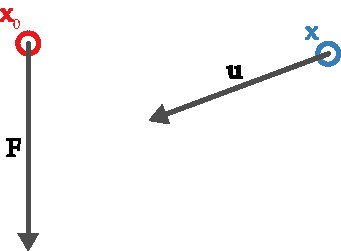
\includegraphics[width=0.3819660112501450000000\textwidth]{img/stokeslet.pdf}
  \caption{Singular point force embedded in stokes flow.}
  \label{fig:stokeslet}
\end{figure}

Additionally, we will later need higher order fundamental solutions which can be obtained by simply differentiating the Stokeslet, e.g. the so-called doublet is defined as
\begin{equation}
  \label{eq:doublet}
  \mathbf{D}(\mathbf{r}) = \frac{1}{2} \Delta\mathbf{S}(\mathbf{r}) = \frac{1}{8\pi\mu} \left(\frac{\mathbf{I}}{|r|^3} - \frac{3rr}{|r|^5}\right) \text{.}
\end{equation}

\section{Boundary integral formulation}

Using the Stokeslet from equation~\eqref{eq:stokeslet} we can now model the influence of an immersed object on the Stokes flow. For a given point $y$ as well as the the force distribution $f$ on the surface of the object we can now calculate the resulting velocity at any point in the flow. The velocity $u$ at the oberservation point $x$ is then given by
\begin{equation}
  \label{eq:boundary_integral_formulation}
  u_i(\mathbf{x}) = \frac{1}{8\pi\mu}\int_{\Omega}S_{ij}(\mathbf{x},\mathbf{y})f_j(\mathbf{y}) \, dS \text{,} \quad i=1,2,3\text{,}
\end{equation}
which is illustrated in Figure~\ref{fig:immersed}.

\begin{figure}[!htbp]
  \centering
  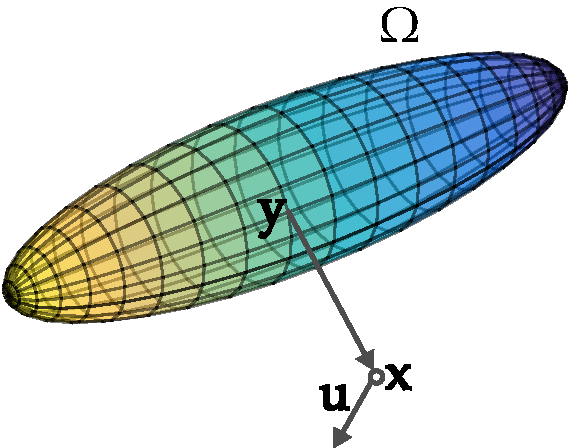
\includegraphics[width=0.3819660112501450000000\textwidth]{img/immersed.pdf}
  \caption{Immersed object in stokes flow.}
  \label{fig:immersed}
\end{figure}

Thus if $f$ is known on the one hand the velocity field can be solved for any point $x$ in the flow which is on the boundary or outside the object. If on the other hand only $u$ is known on the boundary of the object we have to solve the boundary integral integration~\eqref{eq:boundary_integral_formulation}.

However for the simulation we don't know the velocity field $u$ nor do we know the force distribution $f$ on the surface of the object. The only force we know is the externally applied force, which in our case is simply gravity. Additionally we are only concerned with rigid objects. Thus by combining the equations governing rigid body motion with the no-slip boundary condition we can model the velocity field $u$ on the surface $\Omega$ of the rigid body as
\begin{equation}
  \label{eq:rigid_body_motion}
  \mathbf{u}(\mathbf{x}) = \mathbf{U} + \omega \times (\mathbf{x} - \mathbf{x}_c)
\end{equation}
where $\mathbf{x}_c$ and $t$ denote the center point and orientation of the body and $U$ and $\omega$ the translational and rotational velocity respectively. The rigid body motion is illustrated in Figure~\ref{fig:immersed_rigid}.

\begin{figure}[!htbp]
  \centering
  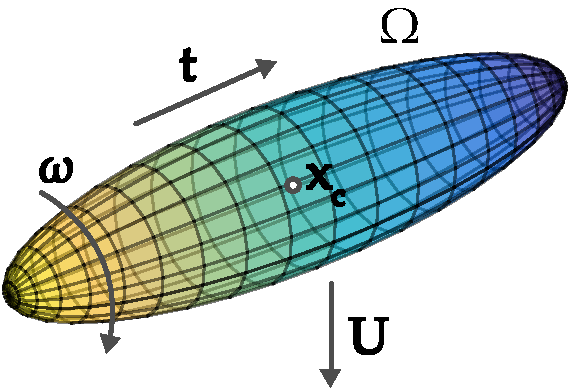
\includegraphics[width=0.3819660112501450000000\textwidth]{img/immersed_rigid.pdf}
  \caption{Immersed object in stokes flow.}
  \label{fig:immersed_rigid}
\end{figure}

Furthermore we required at the integrated force distrubtion over the body as well as the the torque have to be equal to the externally applied force. In our case this is simply gravity and an external torque of $0$. For the a single body the force $\mathbf{F}_{body}$ and torque $\mathbf{T}_{body}$ are thus defined as
\begin{equation}
  \label{eq:force_torque}
  \begin{aligned}
    \mathbf{F}_{body} &= \int_\Omega \mathbf{f}(y) \, dS_y \\
    \mathbf{T}_{body} &= \int_\Omega (\mathbf{x} - \mathbf{x_c}) \times \mathbf{f}(y) \, dS_y \quad i,j=1,2,3\text{,}
  \end{aligned}
\end{equation}

and together with the equation relating the force and velocity for body

\begin{equation}
  \label{eq:boundary_integral_formulation_specific}
  \mathbf{U}_i + (\omega (\mathbf{x} - \mathbf{x}_c))_i = \frac{1}{8\pi\mu} \int_\Omega S_{ij}(\mathbf{x},\mathbf{y} f_i(\mathbf{y}))  \, dS_y
\end{equation}

we obtain the final boundary integral formulation. Until now we only looked at the model for a single body. However for the simulation we want to be able to handle many bodies. By taking advantage of the superposition principle resulting from the linearity of the Stokes equations, the equations \eqref{eq:force_torque} and \eqref{eq:boundary_integral_formulation_specific} can easily be extended.

Reformulating the problem in form of a boundary integral reduced the original 3-dimensional partial differential equation to the 2-dimensional equation over the surface of the body. However for this many-body problem this is still expensive to solve. The next step to reduce the dimensionality of the model simplifies the rigid bodies to slender fibers.

\section{Slender fibers}

The goal of the simulation is to simulate many very slender fibers. For slender fibers the 2D-dimensional boundary integral formulation would be very expensive to solve numerically. We thus simplify the formulation of arbritrary rigid fibers by replacing them with ellipsoids, or more precisly in our case prolate spheroids. They are defined by two parameters, $2*L$ corresponds to the length of the major axis and $a$ to the length of the minor axis or simply the fiber radius.

Additionally, we define the ratio $\epsilon = a / 2 L \ll 1$ and refer to it as the slenderness parameter. As illustrated in Figure~\ref{fig:slenderness}, when $\epsilon$ becomes smaller the shape of the body asymptotically approaches that of an infinitisimal slender fiber.

\begin{figure}[!htbp]
  \centering
  \begin{subfigure}[h]{0.24\textwidth}
    \centering
    \includegraphics[width=\textwidth]{img/slender/1_4.pdf}
    \caption{$\epsilon=1/4$}\label{fig:slenderness_1_4}
  \end{subfigure}
  \begin{subfigure}[h]{0.24\textwidth}
    \centering
    \includegraphics[width=\textwidth]{img/slender/1_10.pdf}
    \caption{$\epsilon=1/10$}\label{fig:slenderness_1_10}
  \end{subfigure}
  \begin{subfigure}[h]{0.24\textwidth}
    \centering
    \includegraphics[width=\textwidth]{img/slender/1_20.pdf}
    \caption{$\epsilon=1/20$}\label{fig:slenderness_1_20}
  \end{subfigure}
  \begin{subfigure}[h]{0.24\textwidth}
    \centering
    \includegraphics[width=\textwidth]{img/slender/1_100.pdf}
    \caption{$\epsilon=1/100$}\label{fig:slenderness_1_100}
  \end{subfigure}
  \caption{Illustration slenderness parameters.}
  \label{fig:slenderness}
\end{figure}

Without this approximation the fundatmental solution have been evaluated on the surface of the rigid body. However, as \cite{} showed the fluid velocity $\mathbf{U}(\mathbf{x})$ at any point $x$ outside the fiber can be also be computed up to an accurary of $O(\epsilon)$ by placing the fundatmental solution on a 1-dimensional fiber centerline. The formulation remains closed for no-slip boundary condition and no angular variation in the fiber velocity.

Thus as shown in Figure~\ref{} each fiber is only defined by its center coordinate and the orientation along its centerline parameterized by the arclength $s \in [-L, L]$. In order to simplify the calculation the rigid fiber simulation uses a non-dimensional formulation of the numerical method. This allows each fiber $m$ to be expressed in terms of
\begin{equation}
  \label{eq:rigid_fiber_model}
  x_m(s,t) = x_m(t) + s * t_m(t) \quad \text{with} \quad s \in [-1, 1] \text{,}
\end{equation}
where $x_m$ is the center cooridnate and $t_m$ the unit tangent vector representing the orientation.

\begin{figure}[!htbp]
  \centering
  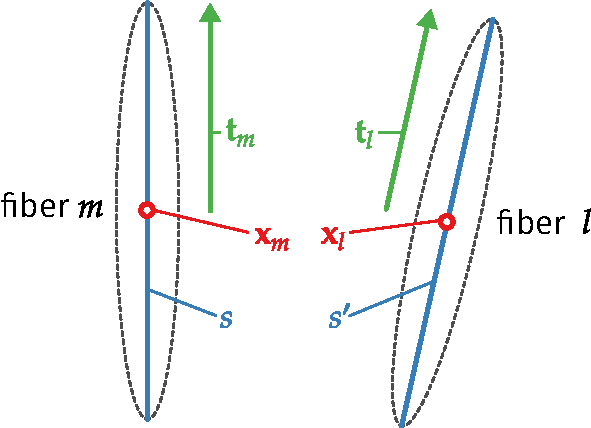
\includegraphics[width=0.3819660112501450000000\textwidth]{img/slender.pdf}
  \caption{Slender fiber approximation.}
  \label{fig:slender_fiber}
\end{figure}

By approximating the slender bodies using slender fibers we can reduce the dimensionality of the boundary formulation from 2D to a 1D integral equation. This allows for a much cheaper numerical simulation. The next step is to combine the equations~\eqref{eq:boundary_integral_formulation_specific} and ~\eqref{eq:force_torque} with non-dimensionalized rigid fiber model in equation~\eqref{eq:rigid_fiber_model} to arrive at the final mathmatical model of the rigid fiber simulation.

For the slender fiber approximation the velocity for the centerline of fiber $m$ is given by
\begin{equation}
  \label{eq:slender_fibers_velocity}
  \begin{aligned}
    \mathbf{\dot{x}}_m + s \mathbf{\dot{t}}_m &= L(\mathbf{t}_m) \mathbf{f}_m(s) \quad \textit{\tiny{(Local contribution)}} \\
     &\quad + (\mathbf{I} + \mathbf{t}_m \mathbf{t}_m)\bar{\mathbf{K}}[\mathbf{f}_m](s) \quad \textit{\tiny{(Global contribution)}} \\
     &\quad + \sum_{\substack{l = 1\\l \neq m}}^M \int_{-1}^{1}\mathbf{G}(\mathbf{R}(s,s'))\mathbf{f}_l(s') \,ds' \quad \textit{\tiny{(Contribution from other fibers)}} \\
  \end{aligned}
\end{equation}
where $\mathbf{\dot{x}}_m$ and $\mathbf{\dot{t}}_m$ denote the translational and rotational velocity of the fiber, respectively. In this equation we take advantage of the superpositon principle in the Stokes flow and simply sum up the contribution over every other fiber $l$ to the current fiber $m$. So for the contribution from another fiber $l$ we integrate over the Stokeslet and Doublet over the complete fiber length for $s' \in [-1, 1]$. The function $\mathbf{G}$ than simply describes a linear combination of the two fundamental solutions
\begin{equation}
  \label{eq:G}
  \mathbf{G}(\mathbf{R}) = S(\mathbf{R}) + \epsilon^2 \mathbf{D}(\mathbf{R}) \text{.}
\end{equation}

By discretizing the integral with a quadrature rule we can calculate the equation~\eqref{eq:slender_fibers_velocity} for a specific number of quadrature points along each fiber. In this case the following function
\begin{equation}
  \label{eq:fiber_distance}
  \mathbf{R}(s, s') = \mathbf{x}_m + s \mathbf{t}_m - (\mathbf{x}_l + s'\mathbf{t}_l) \text{,}
\end{equation}
simply compute the difference vector between the two points on the fiber. Figure~\ref{fig:fiber_contribution} illustrates the case of only two fibers with $5$ quadrature points each.
\begin{figure}[!htbp]
  \centering
  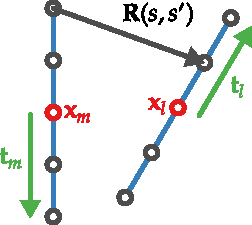
\includegraphics[width=0.3819660112501450000000\textwidth]{img/fiber_contribution.pdf}
  \caption{Contribution between fibers.}
  \label{fig:fiber_contribution}
\end{figure}

Right now we have the we have only one equation but three unknowns. The translational velocity $\mathbf{\dot{x}}_m$, the rotational velocity $\mathbf{\dot{t}}_m$ and the force $\mathbf{f}_m$ acting on the fibers. To close the system we again constrain the force and the torque for each fiber as
\begin{equation}
  \label{eq:force_torque_2}
  \begin{aligned}
    \mathbf{F}_{m} &= \int_{-1}^{1} \mathbf{f}(s) \, ds = \mathbf{F}_g \\
    \mathbf{T}_{m} &= \int_{-1}^{1} s(\mathbf{t}_m \times \mathbf{f}_m(s)) \, ds = 0\text{.}
  \end{aligned}
\end{equation}

The total force integrated over each discretized quadrature point is always equal to the externally applied force, which as discussed before is just gravity. For the torque the same principle applies, however instead of an external influence we always force it to $0$. Together with this the system is now closed and we can solve our rigid fiber simulation using the equations~\eqref{eq:slender_fibers_velocity}~and~\eqref{eq:force_torque_2}.

\chapter{Numerical algorithm and serial implementation}
\label{cha:serial_implementation}

In the last chapter we presented the theoretical foundation of the physics and mathematics involved in simulating rigid fibers. It how Based on the Stokes Equation, it showed how a framework can be developed to efficiently model rigid fibers.

Using this background we will now introduce the approach used for the numeric simulation. Additionally we will touch upon implemtentation details used in the original serial version of the algorithm.

We will seperate the algorithm into four steps and discuss each individually. We close this chapter with a brief reflection of performance characteristica of the serial implementation in order to guide the new parallel implementation on the GPU.

\section{Assemble System}
In the previous chapter we obtained the final closed system and the equations~\eqref{eq:slender_fibers_velocity}~and~\eqref{eq:force_torque_2}. By integrating equation~\eqref{eq:slender_fibers_velocity} from $-1$ to $1$ we can derive two seperate equations for $\mathbf{\dot{x}}_m$ and $\mathbf{\dot{t}_m}$. Using these two equations and some algebra we can obtain a system of equations for $\mathbf{f}_m$ for all fibers from $1,\dots,M$, which only include computable quantities. For more details and an in depth discussion please refer to \cite[].

In order to be able solve these equations for $\mathbf{f}_m$ we have to discretize them. For this we expand the force as a sum of $N+1$ Legendre polynomials $P_n(s)$
\begin{equation}
  \label{eq:force_discretization}
  \mathbf{f}_m = \frac{1}{2}\mathbf{F}_g + \sum_{n=1}^{N}a_{m}^{n} P_n(s) \text{,}
\end{equation}
where the coefficents $a_{m}^{n}$ are vectors with three components. The number of legendre polynomials $N$ used for the force expansion is a parameter and is usually set to $5$ in our simulation.

\subsection{Closed linear system}

Using the force expansion from equation~\ref{eq:force_discretization} in equation~\ref{} we obtain a closed linear system of equations for the coefficents $a_{m}^{n}$ for $n=1,\dots,N$ force expansions and $m = 1,\dots,M$ fibers.

For 3-dimensional positions of the fibers this results in linear system of size $3MN\times3MN$. The first of the algorithm is thus to compute and assemble the linear system in memory. Writing the system the standard form $\mathbf{A}\mathbf{\bar{a}}=\mathbf{b}$ gives the following structure for the matrix $A$
\begin{equation}
  \label{eq:matrix_structure}
  \renewcommand\arraystretch{1.5}
  \mathbf{A} =
  \begin{bmatrix}
    \mathbf{I} & \bar{A}_{12} & \cdots & \bar{A}_{1M} \\
    \bar{A}_{21} & \mathbf{I} & \cdots & \bar{A}_{1M} \\
    \vdots & \vdots & \ddots & \vdots \\
    \bar{A}_{M1} & \bar{A}_{M2} & \cdots & \mathbf{I}
  \end{bmatrix} \text{.}
\end{equation}
In this notation $\bar{A}_{ml}$ describes the $3N\times3N$ matrix encapsulating the contribution from the the force coefficents on fiber $l$ on to the force coefficents for fiber $m$.

\subsection{Inner integral}

For each $\bar{A}_{ml}$ we need to compute the $3\times3$ matrix $\Theta_{lm}^{kn}$
\begin{equation}
  \label{eq:inner_integral}
  \Theta_{lm}^{kn} = \int_{-1}^{1} \left[\int_{-1}^{1}\mathbf{G}(\mathbf{R}(s,s')) P_k(s') \, ds' \right]P_n(s) \, ds \text{,}
\end{equation}
for each force index $k,n = 1,2,\dots,N$ which integrate the legendre polynomials along each fiber. $G$ and $R$ are defined as in equation~\eqref{eq:G}~and~\eqref{eq:fiber_distance}, respectively. Both the inner and the outer integral have to be evaluated for each fiber pair. This can achieved by using a standard gaussian quadrature approach for both the outer as well as the inner integral. However, as fibers get very close the number of quadrature points have to increase to accurately compute the integrals.

Another option is to solve find an analytical solution for inner integral and only solving the outer integral numerically. We will not discuss the detailed derivation for the integral, however for in depth explanation please see \cite[]. One potential downside , of the obtained recursive formulas is their sensitivity due to round off errors. The original serial implementation switches the direction of the recursion, depending on how far apart the fibers are, to minimize this effect.

Choosing between a numerical evaluation for both integral and an analytical integration of the inner integral and numerical integration of the outer integral is a tradeoff between performance and accurary. Inline with the original paper we use a three-point gaussian quadrature rule for each of $8$ subintervals along the integration interval. In total these are than $3 \times 8 = 24$ quadrature points for each integral. The original serial implemention by default evalutes the using the combined numerical and analytical approch for evaluation citing performance benefits. We will later explore how is applies to the new parallel GPU implementation.

\section{Solve System}

After having assembled the linear system $\mathbf{A}\mathbf{\bar{a}}=\mathbf{b}$ the next step is solving it. This can be achieved using standard linear equation solvers. This step is treated as a black box by the simulation, simply plugging in the matrix $\mathbf{A}$ and the vector $\mathbf{b}$ and getting back the solution vector $\mathbf{\bar{a}}$ representing the force coefficients.

The linear system can either be solved using a direct solver or an iterative method like GMRES. Unfortunately the matrix is neither symmetric nor sparse so we can't take advantage of specialized solver for these cases. As long as the fibers are sufficiently far apart and the matrix is not ill-conditioned, GMRES is able to solve the system $<10$ iterations. This is reason why the original serial implementation uses GMRES by default. We will later compare both direct solver as well as iterative solver on the GPU.

\section{Update Velocities}

The force coefficients obtained by solving the linear system can now be used to calculate the remaining unknowns. By using the force expansion in the two seperate equations for $\mathbf{\dot{x}}_m$ and $\mathbf{\dot{t}_m}$. The required implementation is thus similar to the computations for the \emph{Assemble System} step. The two integral, again, can be evaluated either exclusively numerical or with the combined approach of solving the inner integral analytically.

\section{Update Fibers}

The final step takes care of advancing the fibers forward in time. The equations do not impose any strict stability restriction so an explicit time-stepping scheme can be used. We also use the same second order multi-step method used in the original paper. The update for position of the center coordinate $\mathbf{x}_m$ is given by the following discretization in time
\begin{equation}
  \label{eq:time_discretization}
  \frac{3\mathbf{x}_m^{i+1} - 4\mathbf{x}_m^{i} + \mathbf{x}_m^{i-1}}{2 \Delta t} = (2\mathbf{\dot{x}}_m^{i} - \mathbf{\dot{x}}_m^{i-1}) \text{,}
\end{equation}
where the time step is denoted by $\Delta t$ and superscripts denote the numerical approximation of $\mathbf{x}_m(t_i)$. In order to compute the next state this method requires both the previous as well as the current state. So for the first time step $\mathbf{x}_{m}^{1}$ is computed by a simply first order forward Euler method. The calculation for the orientation vector $\mathbf{x}_m$ is almost identically by simply replacing the translational velocity $\mathbf{\dot{x}}_m$ with the rotational velocity $\mathbf{\dot{t}}_m$. Additionally however, we must also renormalize the orientation vector so that it maintains its unit length.

At the end of this step the state of the fibers can be written to an external file for post processing and visualization in other tools. After completing this step the algorithm starts the top again with the \emph{Assemble System} step. This cycle repeats until a specified number of timesteps have been executed.

\section{Algorithm summary}

The original paper implemented this algorithm using Fortran. The computation were all performed in double precision and executed using a single thread on the CPU. In summary the four steps of the algorithm are
\begin{enumerate}
  \item Assemble System
  \item Solve System
  \item Update Velocities
  \item Update Fibers
\end{enumerate}

Emperical results show that the majority of the required computation time is spend on the 1.~\emph{Assemble System} and 2.~\emph{Solve System}. Especially the time required for advancing in step 4.~\emph{Update Fibers} is completely neglible. We will see later in chapter~\ref{cha:benchmarks} that the same holds true for the new parallel implementation.

As the 2.~\emph{Solve System} step is treated as a black box the only potential performance difference is caused by the choice of linear solver. In line with the original paper we will both test direct solver as well as iterative solver like GMRES. However, the short of writing our own implementation of linear solvers on the GPU we have no influence on the performance of this step. We instead of to rely on pre-existing libraries.

Thus the most important step to optimize is 1.~\emph{Assemble System}. Fortunately it is well suited for parallelization. The fibers can naturally partitioned across the compute units, where each unit is responsible for a subset of fibers. The focus of the optimization will thus lie on the \emph{Assemble System}. As the required computation for the 3.~\ref{Update Velocities} step is similar it will also indirectly benefit from any optimizations. Additionally, we will also look at how the two different methods for solving the integral in equation~\ref{eq:inner_integral} perform in the parallel environment. The next goal thus is to parallelize each algorithm step on the GPU.

\chapter{GPU Programming}
In the previous chapter the serial implementation of the numerical simulation was presented. It discussed various implementation details which have to be considered to arrive at the most efficent implementation.

Based on the previous existing serial Fortran implementation this chapter will look at the algorithm in more detail and show, how it was adapted to take advantage of multi-core architectures. Modern GPUs in particular offer a massively parallel architecture and this is why the main focus of this thesis is the implementation of the simulation on a modern nVidia GPUs using CUDA. In addition to the main work of reimplementing the algorithm for CUDA and to have a better understanding of the achievable performance improvements the finished GPU code was also ported to multi-core CPUs using the OpenMP framework.

I will begin with a short introduction to general purpose computing on the GPU and explain briefly how CUDA works. I then move on to illustrate the practical implementation of the CUDA code. This is followed by a brief explanation of OpenMP and how the code was parallelized on the CPU. The chapter ends with the discussion of several potential optimization approaches to further improve the performance of the simulation.

\section{Overview}
In the beginning of Graphics Processing Units were highly specialized pieces of hardware developed to exclusively improve the performance of real-time 3D graphics. However, in recent years GPUs have started to be able to run arbitrary code instead of being limited to graphics related computations. This allows them to achieve impressive performance increases across a wide range of different general purpose applications. The deciding factor is how well the problem can be parallized to take advantage of the massively parallel architectures of GPUs. This has lead to potentially large performance advantages of GPUs over CPUs as illustrated in figure~\ref{fig:gpu_performance}. It shows the year over year increase in the theoretical floating point operations per second (GFLOP/s). The FLOP/s number is calculated by combining information of the number of compute cores, core frequency and memory bandwidth for both the CPU and GPU models. This does not necessarily translate to direct real world performance increases but tries to show the potential GPUs have.

\begin{figure}[!htbp]
  \centering
  \begin{tikzpicture}
    \setmathfont{FiraSans-Book.otf}
    \begin{axis}[
      title=Theoretical GFLOP/s,
      xlabel={Year},
      ylabel={GFLOP/s},
      date coordinates in=x,
      xticklabel={\year},
      date ZERO=2002-01-01,
      xtick={2002-01-01,2004-01-01,2006-01-01,2008-01-01,2010-01-01,2012-01-01,2014-01-01},
      xmin=2002-01-01,
      xmax=2014-01-01,
      ymin=0,ymax=5500,
      ]
      \addplot[color=set12_light,mark=*,mark options={fill=white}, very thick] table[x=Date,y=Double,col sep=comma,meta=Name] {charts/cpu_performance.csv};
      \addlegendentry{Intel CPU Double Precision}

      \addplot[
      scatter,
      visualization depends on=\thisrow{alignment} \as \alignment,
      nodes near coords,
      point meta=explicit symbolic,
      every node near coord/.style={anchor=\alignment},
      color=set13_light,
      mark=*,
      mark options={fill=white},
      very thick,
      every node near coord/.append style={font=\tiny},
      ] table[x=Date,y=Double,col sep=comma,meta=Name] {charts/double_gpu_performance.csv};
      \addlegendentry{NVIDIA GPU Double Precision}

      \addplot[
      scatter,
      visualization depends on=\thisrow{alignment} \as \alignment,
      nodes near coords,
      point meta=explicit symbolic,
      every node near coord/.style={anchor=\alignment},
      color=set12,
      mark=*,
      mark options={fill=white},
      very thick,
      every node near coord/.append style={font=\tiny},
      ] table[x=Date,y=Single,col sep=comma,meta=Name] {charts/cpu_performance.csv};
      \addlegendentry{Intel CPU Single Precision}
      \addplot[
      scatter,
      visualization depends on=\thisrow{alignment} \as \alignment,
      nodes near coords,
      point meta=explicit symbolic,
      every node near coord/.style={anchor=\alignment},
      color=set13,
      mark=*,
      mark options={fill=white},
      very thick,
      every node near coord/.append style={font=\tiny},
      ] table[x=Date,y=Single,col sep=comma,meta=Name] {charts/single_gpu_performance.csv};
      \addlegendentry{NVIDIA GPU Single Precision}

    \end{axis}
    \setmathfont{XITS Math}
  \end{tikzpicture}
  \caption{Increase in floating-point operations per second for CPUs versus GPUs over time.}
  \label{fig:gpu_performance}
\end{figure}

The huge difference in performance mainly derives from the number of independent compute cores. Even though each individual core of a traditional CPU is very fast they usually only have four, eight or maybe sixteen cores. In contrast to this GPUs can have several hundreds of indepedent compute cores. Each core can simulatenously perform calculations and thus provides the opportunity to yield big performance improvements for high-throughput type computations. This fact also introduced general purpose computing on GPUs to the world of supercomputers. Over time, a growing number of them started supplimenting their compute power with GPUs and some even rely exclusively on GPUs for their computations.

In order to take advantage of these new massively parallel architectures new Application Programming Interfaces (API) had to be developed. The two proposed APIs are OpenCL and CUDA. OpenCL is an open and cross platform standard maintained by the Khronos Group. The same group is also responsible for its graphics focused counterpart OpenGL. OpenCL is not exclusive to GPUs, but instead tries to be a general abstract layer for different parallel architectures. This allows OpenCL code to be run not only on GPUs but also on CPUs and other new hardware like Intels Xeon Phi. CUDA on the other hand is developed by Nvidia exclusively for their line of GPUs.

Choosing between OpenCL and CUDA is the first decision to be made when starting to implement a new project on GPUs. The main advantage of OpenCL is the ability to be able to run on many different devices. All major players in the computing space provide an implentation on top of their platforms. Both Intel and AMD provide the API for their CPU and both AMD and Nvidia have drivers available for their GPUs. However, this advantage can also be a disadvantage as the achievable performance might suffer from the abstraction across all platforms. The OpenCL framework is potentially not optimized for a particular device specific architecture. CUDA on the contrary is in theory highly optimized to achieve the best possible performance on Nvidia's GPUs. In practice the difference can possibly be mitigated by spending the extra time to fine-tune the OpenCL implementation to the hardware's specific needs. Another disadvantage of OpenCL is the potentially outdated and inconsistent driver support for the various devices. This is especially true for Nvidia who seem to have stopped updating OpenCL, still only supporting OpenCL 1.1 which was released back in 2010. Their main focus is on pushing CUDA and updating it to support all the feature in their new GPUs.

For this thesis I chose to go with Nvidia's CUDA framework mainly because of the available hardware both at the workstation computers as well as at the local computing cluster. Additionally this project does not need the cross-platform capability as the main focus is on pure performance in a highly specialized setup and simulation scenario. The application will not be widely distributed and only used for internal purposes.

\section{CUDA}
\label{sec:CUDA}
The CUDA stands for Compute Unified Device Architecture and was introduced by Nvidia in 2006 as a general purpose parallel computing platform. It leverages the highly parallel architecture of modern Nvidia GPUs to solve many different computational problems, which can lead to potentially large performance improvements compared to traditional CPUs.

The CUDA platform allows developers to use a variety of different options to program the GPU. The easiest way is to link to any CUDA-accerlated library and simply using the libraries interfaces from any software environment. For more advanced uses extensions to various programming languages exist like C/C++, Fortran and even managed languages like Java and Python and many more. This allows for easy and fast integration into any software environment the developer is comfortable with. figure~\ref{fig:cuda_overview} illustrated the different components of the overall CUDA platform.

\begin{figure}[!htbp]
  \centering
  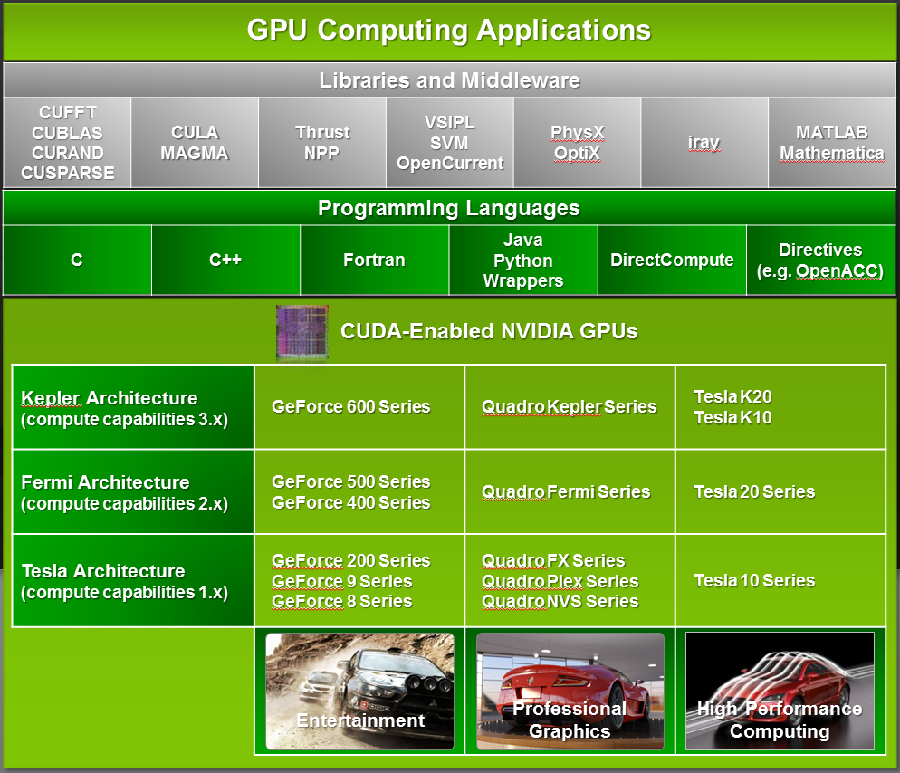
\includegraphics[width=\textwidth]{img/cuda_overview.pdf}
  \caption{Overview of the CUDA platform.}
  \label{fig:cuda_overview}
\end{figure}

The basic building blocks of the CUDA Programming Model from a development perspective are kernels. CUDA kernels are the equivalent of normal C functions. However the major difference is that instead of being executed just once, kernels are executed in parallel by $N$ different threads. These CUDA threads are distributed and run across the available compute cores of the GPU. To illustrate how a very basic kernel call looks, figure \ref{lst:code_vector_addition} shows a code sample for a very simple vector addition.

\begin{listing}[!htbp]
  \centering
  \begin{minted}[mathescape,
    linenos,
    numbersep=5pt,
    fontsize=\footnotesize,
    frame=lines,
    framesep=2mm]{c}
// Kernel definition
__global__ void VecAdd(float *A, float *B, float *C)
{
  int i = threadIdx.x;
  C[i] = A[i] + B[i];
}

int main()
{
  ...
  // Kernel invocation with N threads
  VecAdd<<<1,N>>>(A,B,C);
  ...
}
  \end{minted}
  \caption{Pseudocode for CUDA vector addition}
  \label{lst:code_vector_addition}
\end{listing}

\paragraph{CUDA Kernels}

It is important to remember that each kernel invocation is executed independently and no ordering is guaranteed. It is therefore essential to make sure to avoid any race conditions or shared memory access. There are however, ways to allow for shared memory access which will be briefly touched upon later in the practical implementation of the simulation.

\paragraph{Thread hierarchy}

In order to efficiently distribute the different threads across the compute cores of the GPU, CUDA defines a thread hierachy. As discussed previously a GPU consists of many independent compute cores. On Nvidia GPUs theses cores are referred to as Streaming Multiprocessors (SMs). During execution of the application each SM is tasked with running a distinct set of threads. In CUDA these sets of threads are called thread blocks. Each thread block is then distributed to all the available SMs, which allows for automatic scalability depending on the number of SMs available  as illustrated in figure~\ref{fig:automatic_scaling}.

\begin{figure}[!htbp]
  \centering
  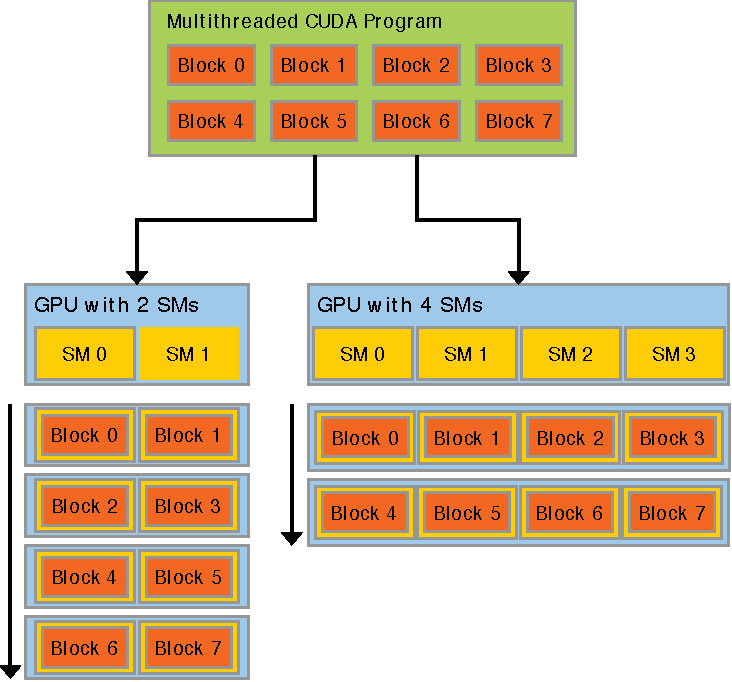
\includegraphics[width=\textwidth]{img/automatic_scaling.pdf}
  \caption{Automatic scaling of blocks across an arbitrary number of Streaming Multiprocessors.}
  \label{fig:automatic_scaling}
\end{figure}

Thus the developer only has to divide the workload into appropriately sized blocks of threads and invoke the kernel. How to choose the optimal size of a block to maximize the performance is not an easy question to answer and is highly dependent on the particular task and implementation. In practice the size is often chosen by running benchmarks with various different sizes to determine the sweet spot.

In order to make programming and modeling of real world problems easier CUDA blocks can be addressed using either a one-dimensional, two-dimensional, or three-dimensional thread index. For example in the case of a matrix calculation it is more natural to think about parallelizing each element given by the row and column index instead of a single one-dimensional index. This is illustrated in the code simple in listing~\ref{lst:code_matrix_addition}

\begin{listing}[!htbp]
  \centering
  \begin{minted}[mathescape,
    linenos,
    numbersep=5pt,
    fontsize=\footnotesize,
    frame=lines,
    framesep=2mm]{c}
// Kernel definition
__global__ void MatAdd(float A[N][N], float B[N][N], float C[N][N])
{
  int i = threadIdx.x;
  int j = threadIdx.y;
  C[i][j] = A[i][j] + B[i][j];
}

int main()
{
  ...
  // Kernel invocation with one block of N * N * 1 threads
  int numBlocks = 1;
  dim3 threadsPerBlock(N, N);
  MatAdd<<<numBlocks, threadsPerBlock>>>(A,B,C);
  ...
}
  \end{minted}
  \caption{Pseudocode for CUDA matrix addition, illustrating 2D thread blocks}
  \label{lst:code_matrix_addition}
\end{listing}

Finally because the resources of each Streaming Multiprocessor are limited there exists a upper bound of how many threads a block can contain. Currently this maximum number of threads is $1024$. This means that the maximum size of matrices possible to be added in the code sample in listing~\ref{lst:code_matrix_addition} is $32\times32$. To solve this problem CUDA introduces another layer above blocks called a grid. A grid organizes thread blocks again into either one, two, or three dimensions. The number of thread blocks in a grid is unlimited and thus solely dependent on the size of the workload. Listing~\ref{fig:grid_blocks} shows an example configuration of a 2D grid with 2D blocks.

\begin{figure}[!htbp]
  \centering
  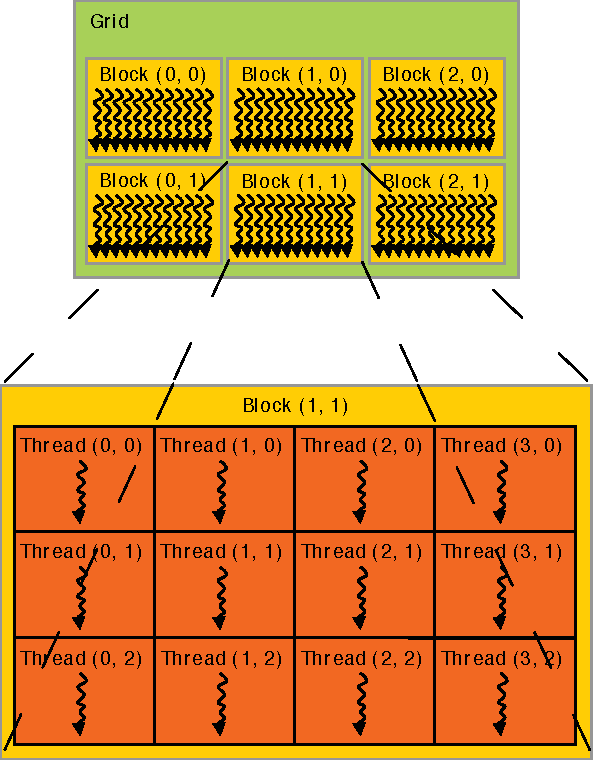
\includegraphics[width=0.6\textwidth]{img/grid_blocks.pdf}
  \caption{Overview of the CUDA platform.}
  \label{fig:grid_blocks}
\end{figure}

\paragraph{Memory hierarchy}

In addition to the Thread hierarchy...

\begin{itemize}
\item 4 Layers, Global, Local, Private
\item Global shared across all SM
\item Local shared across thread block
\item Private per thread
\item Latency VERY different between layers
\item Avoid global memory access
\item Or hide with compute heavy, as is the case with assemble system step (ala will be used later)
\end{itemize}

\chapter{Parallel Implementation}

\section{Development environment}

The rigid fiber simulation developed as part of this thesis is only loosely based on the original serial Fortran implementation. This was done to ensure a clean starting point and avoid difficulties in adapting the existing code for parallel execution as it was never intended to be run across multiple cores. This also provided the opportunity to learn from the shortcomings of the old code to not only parallelize it but also improve the efficiency in general.

The development was done exclusively on a Linux workstation running Ubuntu as this will also be the exact same runtime environment used in the later experimental usage of the resulting application. The build system for compiling and linking the final application was CMake. It was chosen because it is widely used open-source and cross-platform build system, which allowing for easy integration of the various required libraries in a well documented and straightforward manner.

Under the hood the build system uses Nvidia's CUDA platform tools to compile the code. For this Nvidia includes \emph{nvcc}, an LLVM-based CUDA compiler capable of compiling C/C++ code together with the CUDA specific extensions. In addition to the CUDA platform, the application also requires support libraries for the different linear solvers. The two main libraries are \emph{MAGMA} for the direct solver and \emph{ViennaCL} for the iterative solvers. Both will be introduced briefly now.

\paragraph{MAGMA / CuBLAS / OpenBLAS}
The MAGMA project contributes the implementation for the direct solver used in this thesis. This dense linear algebra library provides features similar to standard LAPACK functions but for multicore architectures. It also has features to support hybrid algorithms to run code across multiple GPUs or CPUs at the same time, however these features were not explored in this thesis. Instead the focus was on a high performant single GPU implementation of a direct linear system solver.

MAGMA provides the interfaces for various high-level languages, however the underlying math functions utilize the platform specific implementations of the BLAS levels. For CUDA this is implemented directly by Nvidia in the form of the CuBLAS libraries. Additionally, MAGMA tries to be as fast as possible which sometimes means integrating CPU based algorithm where it is has performance advantages. Thus a CPU based BLAS implementation is also needed. For this the OpenBLAS library was chosen which is the most up-to-date and high performant library available outside the very expensive Intel MKL library. OpenBLAS takes full advantage of multicore systems using pthreads and is also used for the comparison of Fortran CPU implementation against the CUDA GPU implementation

\paragraph{ViennaCL}
ViennaCL is an open-source linear algebra library developed at the Universiy of Vienna. The library provides an abstraction layer across many different parallelization methods in order to facilitate consistent and easy to use support for BLAS level 1-3 and iterative solvers. This unique feature allows the developer to easily switch between different backends for parallelization. Currentely, the library supports OpenMP, OpenCL and most importantly for this thesis - CUDA.

ViennaCLs focus is on solving sparse matrices with the implemented iterative solvers. However, it also has basic support for solving dense matrices using a variety of different iterative solvers. As the rigid fiber simulation exclusively relies on dense matrices this makes it an ideal candidate for benchmarking. For this thesis both the BiCGStab as well as the GMRES iterative solvers where used and tested.

In order to faciliate easier usage of the application both during development and later real-world usage a Python wrapper script is also available. The script completely automates the building process and dynamically customizes the application code to support three different modes of operation. The first is a simple \emph{run} mode which takes the supplied parameters and executes the simulation. The second mode is \emph{validate}, it allows for a fully automated way to test and validate different algorithm variations against a known correct simulation run. This includes automatically computing the error as well as the error location in the matrix allowing for easier debugging of changes. The last mode is \emph{benchmark} which runs the supplied parameters through a series of iterations collecting and aggregating timings for each simulation step as well as the total time.

\begin{itemize}
\item Unified interface for OpenMP and CUDA -> OpenMP only introduced later... -> Is that really important any way?
\end{itemize}

\section{Kernels}
The overall parallel algorithm is very similar to the serial version, however, each simulation step is seperated into different kernels. Each kernel is invoked in a serial manner, this means CUDA guarantees that all data modified in a kernel is available before the next kernel is executed. These kernels are then distributed across the GPU. All calculations are done using single precision floating point numbers, as Nvidia limits high performance double precision computation to their server class GPUs. The CUDA pseudocode for the algorithm is illustrated in listing~\ref{lst:pseudo_parallel_algorithm}. It begins by parsing by parsing the simulation parameters and the initial fiber configuration. After that, the required memory is allocated on the GPU. Finally a simple loop executes all timesteps and for each step the four main algorithm substeps — 1. \emph{Assemble System}, 2. \emph{Solve System}, 3. \emph{Update Velocities} and 4. \emph{Update Fibers} — are run on the GPU.

\begin{listing}[!htbp]
  \centering
  \begin{minted}[mathescape,
    linenos,
    numbersep=5pt,
    fontsize=\footnotesize,
    frame=lines,
    framesep=2mm]{c}
int main()
{
  // Parsing algorithm parameters and initial fiber positions
  readParameters();
  readFiberConfiguration();
  allocateGPUMemory();
  ...

  for (int step = 0; step < max_timestep; step++)
  {
    AssembleSystem<<<numBlocks, threadsPerBlock>>>(...);
    SolveSystem<<<numBlocks, threadsPerBlock>>>(...);
    UpdateVelocities<<<numBlocks, threadsPerBlock>>>(...);
    UpdateFibers<<<numBlocks, threadsPerBlock>>>(...);
  }
  ...
}
  \end{minted}
  \caption{Pseudocode for parallel algorithm on the host.}
  \label{lst:pseudo_parallel_algorithm}
\end{listing}

The application requires two general configuration files as an input. The first file is referred to as the parameters file which contains the different configuration variables and constants used throughout the algorithm. These include, for example the number and size of the timesteps as well as the number of force expansion terms and number of quadrature points. Additionally, this file is also used to configure the iterative solvers like specifiying the number of restarts for GMRES or the solution tolerance for BiCGStab and GMRES.

Each of the parallelized substeps are now discussed in more detail. The purpose of each kernel as well as the required input and outputs.

\paragraph{Assemble System}

\begin{listing}[!htbp]
  \centering
  \begin{minted}[mathescape,
    linenos,
    numbersep=5pt,
    fontsize=\footnotesize,
    frame=lines,
    framesep=2mm]{c}
__global__ void AssembleSystem1D(
  in float *positions,
  in float *orientations,
  out float *a_matrix,
  out float *b_vector)
{
  const int i = blockIdx.x * blockDim.x + threadIdx.x;

  if (i >= NUMBER_OF_FIBERS) return;

  for (int j = 0; j < NUMBER_OF_FIBERS ++j)
  {
    for (int force_index_j = 0;
         force_index_j < NUMBER_OF_TERMS_IN_FORCE_EXPANSION;
         ++force_index_j)
    {
      computeInnerIntegral(...);

      for (int force_index_i = 0;
           force_index_i < NUMBER_OF_TERMS_IN_FORCE_EXPANSION;
           ++force_index_i)
      {
        // Only 1D thread block
        // Each thread updates unique memory locations, thus
        // no need for atomics
        setMatrix(...)
        setVector(...)
      }
    }
  }
}
  \end{minted}
  \caption{Pseudocode for the assemble system step with a 1D thread block.}
  \label{lst:pseudo_assemble_system}
\end{listing}

The \emph{Assemble System} kernel is the most important step of the algorithm. Its goal is to build the matrix and vector in memory for the linear system of equations in the form of $A*x = b$. Listing~\ref{lst:pseudo_assemble_system} shows the pseudocode for the one-dimensional implementation of the assemble system step. This means the code is parallelized for each fiber and each thread calculates the contributions to this fiber from all other fibers. Looking at the matrix each thread is thus responsible for $3*M$ rows of the matrix.

The kernel requires two inputs, the current position of each fiber and its orientation. Using these combined with the equations outlined in chapter~\ref{cha:theoretical_foundation} and chapter~\ref{cha:serial_implementation} the matrix and vector elements are computed and used in the next step to solve the linear system they define.

\paragraph{Solve System}
As this thesis does not aim to implement generic linear solvers, this step is treated as a black box. During the previous \emph{Assemble System} kernel two arrays containing the matrix and right hand side of the linear system have been computed. These two arrays are now passed to the respective function of the library containing the linear solver. This is the MAGMA library in case of the direct solver and the ViennaCL library in case of the two tested iterative solvers BiCGStab and GMRES. Both libraries are able to directly use the already allocated memory regions and no additional allocations have to be performed. In order to conserve memory space the resulting solution vector is stored in the same memory location as the $b$-vector and is passed on to the subsequent steps.

\paragraph{Update Velocities}

\begin{listing}[!htbp]
  \centering
  \begin{minted}[mathescape,
    linenos,
    numbersep=5pt,
    fontsize=\footnotesize,
    frame=lines,
    framesep=2mm]{c}
__global__ void UpdateVelocities2D(...)
{
  const int i = blockIdx.x * blockDim.x + threadIdx.x;
  const int j = blockIdx.y * blockDim.y + threadIdx.y;

  if (i >= NUMBER_OF_FIBERS) return;
  if (j >= NUMBER_OF_FIBERS) return;
  if (i==j) return;

  for (int quadrature_index_i = 0;
       quadrature_index_i < TOTAL_NUMBER_OF_QUADRATURE_POINTS;
       ++quadrature_index_i)
  {
    for (int quadrature_index_j = 0;
         quadrature_index_j < TOTAL_NUMBER_OF_QUADRATURE_POINTS;
         ++quadrature_index_j)
    {
      force = computeForce(coefficents, ...)
      computeDeltaVelocities(force)
    }
  }

  // 2D thread block
  // Each thread responsible for an interaction pair, thus
  // result is written to the same memory location
  // Using atomics to avoid conflicts
  atomicAdd(&(translational_velocities[i].x),
              delta_translational_velocity.x);
  atomicAdd(&(translational_velocities[i].y),
              delta_translational_velocity.y);
  atomicAdd(&(translational_velocities[i].z),
              delta_translational_velocity.z);

  atomicAdd(&(rotational_velocities[i].x),
              delta_rotational_velocity.x);
  atomicAdd(&(rotational_velocities[i].y),
              delta_rotational_velocity.y);
  atomicAdd(&(rotational_velocities[i].z),
              delta_rotational_velocity.z);
}
  \end{minted}
  \caption{Pseudocode for the updating velocities simulation step.}
  \label{lst:pseudo_update_velocities}
\end{listing}

After solving the linear system the solution coefficents are used to update the velocities of the fibers. The \emph{Update Velocities} kernel accumulates the exerted forces for all fibers and updates both the translational as well as the rotational velocities simultaneously. In this particular instance the 2D thread block version of the kernel is illustrated in listing~\ref{lst:pseudo_update_velocities}. This means each individual kernel invocation is responsible for a single pair of fiber interaction. Under the normal assumption that kernel invocations are not allowed to write to the same memory location since this would result in undefined behaviour and incorrect results for the velocities.

Fortunately CUDA provides a mechanism to circumvent this issue. By using so-called atomic function CUDA streamlines and serializes the memory access. Thus the atomicAdd function accumulates different velocity contributions to a fiber from all the other fibers. This ensures that each update to the memory location is handled in a serial manner, guaranteeing the correct value in memory for each. Of course this implies a potential performance degradation, however, newer GPUs with new CUDA version have been very well optimized to only have a minimal negligible impact. Benchmarking for the fibers simulation shows that using a 2D thread block and the associated performance increases far outweight the potential performance hit of using atomics.

\paragraph{Update Fibers}

\begin{listing}[!htbp]
  \centering
  \begin{minted}[mathescape,
    linenos,
    numbersep=5pt,
    fontsize=\footnotesize,
    frame=lines,
    framesep=2mm]{c}
__global__ void UpdateFibers()
{
  int i = blockIdx.x * blockDim.x + threadIdx.x;

  if (i >= NUMBER_OF_FIBERS) return;

  next_positions[i] = 4/3 * current_positions[i]
    - 1/3 * previous_positions[i]
    + 2/3 * TIMESTEP
      * (2 * current_translational_velocities[i]
         - previous_translational_velocities[i]))

  next_orientations[i] = 4/3 * current_orientations[i]
    - 1/3 * previous_orientations[i]
    + 2/3 * TIMESTEP
      * (2 * current_rotational_velocities[i]
         - current_rotational_velocities[i]))

  normalize(next_orientations)
}
  \end{minted}
  \caption{Pseudocode for the updating fibers simulation step.}
  \label{lst:pseudo_update_fibers}
\end{listing}

The final simulation step takes care of advancing the position and orientation of the fibers in time. The pseudecode in listing~\ref{lst:pseudo_update_fibers} implements the second-order multi-step method introduced in section~\ref{sec:time_stepping}. As will be seen later in the results in chapter~\ref{cha:benchmarks} this required time for this kernel is minuscule compared to the other steps. The kernel only scales linearly and in addition has a perfectly aligned memory access resulting in close to optimal usage of the GPU hardware.

\section{Optimizations}
\label{sec:optimizations}

During the development of the parallel GPU simulation great care was taken to continuously optimize the code both on an algorithmic level as well as on an implementation level. Numerous small code-level optimizations have been performed based on the original serial code like precomputing as much data as possible, avoiding variable allocations or unnecessary copy operations in performance critical sections of the code.

Additionally, more advanced optimization were made like rearranging calculations inside loops to avoid executing redundant calculations and consolidating multiple loops into one. Finally, techniques such as loop unrolling and faster math functions where also tested and included.

Throughout the optimization phase the benchmark suite was run after each step. This ensures that optimizations were only included if they had a measureably impact on the overall performance of the simulation. Moreover, in this way potential performance regressions could be identified early and be avoided.

Many optimizations performed during this process are applicable to both the CPU and GPU and show performance improvements for both. However, some optimizations or algorithm variations have either a different effect or are uniquely suited and related to the GPU hardware. For this thesis we will look into three general different optimizations in more detail. The performance results for each will then later be discussed in chapter~\ref{cha:benchmarks}.

\subsection{Numeric vs. Analytic Integration}
\label{subsec:numeric_analytic}
The first optimization was already part of the original serial implementation as described in section~\ref{sec:quadrature}. In the original paper \cite{} the authors observed that the analytical integration of the inner integral yielded a performance increase compared to the numerical integration. On paper an analytical integration should also not only be preferred because of being faster but more importantly also being more accurate.

However, for numerical precision reasons the actual implementation of the analytical integration can't achieve this theoretical level of accuracy. The implementation is dependent on a design variable which uses a slightly different code to calculate the integral for very close fibers in order to avoid numerical instabilities. The computation of the inner integral lies at the heart of the algorithm and is a very performance critical section of the implementation. Exploring the performance implications of both approaches on the GPU is thus of great interest, and especially how it compares against the same algorithm running on the CPU.

\subsection{Shared Memory}

As the described in section~\ref{sec:CUDA} CUDA code is subject to a highly specialized memory hierarchy. Whereas traditional CPUs only have small caches and a large main memory pool, CUDA introduces the concept of a shared local memory space. The access time to this local memory is orders of magnitudes faster compared to accessing the global GPU memory. Additionally, local memory can be shared among a CUDA thread block and potentially save time by avoiding to constantly access the slow global memory.

In order to test this, shared memory was implemented and tested with the \emph{Assemble System} step, the most performance critical kernel written for the fiber simulation. To understand the idea, imagine the 2D thread block implementation of the kernel. Each thread block is responsible for many pairs of fiber interactions, e.g. fibers $[1,8]$ each interacting with fibers $[9,16]$. In total, these are $8 \times 8 = 64$ interactions. Each kernel invocation is responsible for one pair and has to load the position and orientation for the two interacting fibers. However, on closer inspection it is obvious that one does not need to load each fiber every time. As soon as fiber $1$ has been loaded into shared memory it can be reused for all the interactions with fibers $9$ through $16$ avoiding the unnecessary and slow access to global memory.

How this affects performance, however, is not always easy to tell, as various factors can influence the result. If the loaded data is small enough, the various memory caches can hide to increased costs of accessing global memory. Also while the first threads in a thread block load the data from global to shared memory, all other threads in this thread block have to wait for their data to become available. This has a particular large impact when the overall kernel has to execute many calculations and the required time for computations effectively hides the memory loading time. CUDA is than able to seamlessly and very efficiently switch to the next thread block and continue executing it. In this case the performance penalty only occurs at the very beginning and end, and has only a negligible impact on the overall performance.

However, in general efficient exploitation of shared memory can be a huge advantage for parallel GPU implementations. Especially when comparing the performance against CPUs, as they don't have an equivalent fast and comparatively large memory space. It is therefore an interesting optimization to explore and benchmark.

\subsection{Thread Block Dimension}

There are many different factors that determine the performance of a particular GPU algorithm. This is especially true with regards to optimally taking advantage of the specific underlying GPU architecture, which change even between different models of graphics cards. How to best utilize the hardware depends on specific memory access patterns, avoiding too much register usage and choosing optimal settings for the thread block size. Each graphics cards can have a different number of streaming multiprocessors with only limited resources and taking advantage of this can result in performance increases.

For this thesis we looked at the Thread Block dimension in particular and how choosing a different approach of parallelizing affects the performance. Doing so, the focus was on the \emph{Assemble System} step, which is the most performance critical step. However, the results were then also transferred to the \emph{Update Velocities} step.

The most straight forward approach is to simply parallelize the algorithm with regards to a single fiber. This means each kernel invocation is responsible for calculating all the interactions for this fibers with all other fibers. In this way a single kernel is responsible for multiple rows of the resulting linear system matrix. Additionally, this approach does not have any memory access conflict as each kernel only writes to the memory location belonging to its unique fiber. The potential disadvantage for a one-dimensional thread block, however, is that the resulting code can be more resource intensive for each single kernel and potentially hinder the performance on each multiprocessor.

For a two-dimensional thread block each kernel invocation is responsible for a pair of fibers interacting. While this decreases the necesseary resources, it also required atomics which can potential slow down the execution. Three-dimensional thread blocks are the maximum allowed dimensions for a CUDA thread block. They are a further extension of the two-dimensional thread block, as now each kernel invocation is responsible not for the complete interaction but only the interaction resulting from a specific point from the force expansion. This results in even more potential memory conflicts and also increases the total number of thread blocks which have to be distributed.

How exactly each decision for the thread-block dimension affects performance is not clear. Only trial-and-error benchmarking combined with metrics from CUDA can find the optimal setting for the specific algorithm.

\section{OpenMP}

The goal of this thesis is to implement a high performant rigid fiber simulation on the GPU using CUDA. In order to better understand to what degree this goal was achieved, it is crucial to have a comparison. The original serial implementation is not an ideal candidate as it does differ in a number of ways. First of all, its purely serial and doesn't take advantage of todays multicore CPUs. Furthermore, it was implemented in double precision and because of arbitrary restrictions Nvidia places on its consumer GPUs they are only really well suited for single precision. That is why the CUDA implementation is strictly single precision. Finally, the primary focus of the original Fortran implementation was a correctly implemented algorithm and not performance.

For these reasons and in order to have a fairer comparsion of the performance differences between the GPU and CPU implementation, a completely new and rewritten parallel CPU simulation was also implemented. For the parallelization on the CPU the OpenMP library was chosen.

After having implemented a parallel algorithm for the GPU, the conversion to the OpenMP-based CPU implementation was relatively straightforward. All optimizations done for the GPU implementation were also applied to the new CPU code when applicable. In order to parallelize the BLAS functions required for the linear solver the already included OpenBLAS library was chosen. OpenBLAS is an open-source and highly optimized library and automatically parallelizes BLAS functions using pthreads across all available CPU cores. In contrast to the GPU implementation, the OpenMP version is only parallelized in one-dimension. This means that each core calculates the interactions for one fiber with all other fibers or put differently all matrix rows belong to one fiber. As the underlying number of independant threads is much lower on CPUs, different parallelization dimensions didn't have an impact during testing.

The end results of the practical implementation for this thesis is a highly optimized CUDA implementation for Nvidia GPUs and additionally a parallelized and optimized Fortran OpenMP implementation for CPUs. The next chapter will now look at a number of performance metrics and compare them between the GPU and CPU.

\chapter{Benchmarks}
\label{cha:benchmarks}

The last chapter introduced the parallel implementation of the numerical simulation. It presented the concept of general purpose computing on modern GPUs. This was followed with a practical overview of the implementation of the algorithm using Nvidia's CUDA framework. Additionally, possible optimiziations to take advantage of the unique properties of the GPU architecture were outlined.

Using all the available implementations of the algorithm this chapter will showcase a multitude of different results and benchmarks performed. This is done to illustrate the achieved performance increases on the GPU over the original serial CPU implementation and the parallel OpenMP implementation.

\section{Methodology}

The methodology used for the benchmark suite is the same for all presented benchmarks. This ensures comparable results and fairest comparison possible.

\subsection{Hardware}

All benchmarks were run on the same workstation with specifications listed in table~\ref{tab:workstation}. The components were chosen to provide a balanced system.
This was done to come as close as possible to a fair comparison between the CPU and GPU, as comparing a high-end CPU against a low-end GPU would only be of limited value.

\begin{table}[!htbp]
  \begin{center}
  \begin{tabulary}{0.7\textwidth}{LL}
    \toprule
    \multicolumn{2}{c}{Workstation} \\
    \midrule
    Processor & Intel Core i7 4770 \\
    Graphics & Nvidia GTX 970 4GB \\
    RAM & 16GB DDR3 \\
    Operating System & Ubuntu Linux 12.04 LTS \\
    CUDA Driver & CUDA 6.5.xxxx \\
    \bottomrule
  \end{tabulary}
\end{center}
\caption{Benchmark system hardware specification}
\label{tab:workstation}
\end{table}

\subsection{Benchmark scheme}

The main goal of the benchmark system was to generate statistical significant and reproducible performance numbers. To ensure this, all benchmarks for both the GPU and the CPU were run using the exact same scheme like the number of iterations and stop criteria. In order to obtain the timings, the built-in CUDA timing events were used for each individual kernel. For Fortran the \emph{SYSTEM\_CLOCK} function was used respectively.

For all different benchmarks timings were obtained for a different number of fibers starting from $100$ up to $2000$ in $100$ increments. For each seperate number of fibers a number of iterations are run to obtain the average over multiple runs. For each iteration a completely new and random initial fiber configuration is generated with the current number of fibers. In order to exclude illegal configurations where fibers overlap and intersect an additional correction pass is done over the fibers to ensure a minimal and average distance between all fibers. For the configrations in this thesis the minimal distance was always set to $0.2$ and the average to $0.4$ respectively.

Using this semi-random generation the rigid fiber simulation is run for exactly $10$ timesteps. To avoid remaining outliers in the configuration causing potentially large variation in the timings the first timestep is excluded. This is especially true for iterative solvers which are highly dependent on the configuration. The first timestep is thus used as a simple warmup step for the simulation. So the final average time for each run is taken from the last $9$ timesteps.

In order to ensure a statistical significant result, the number of iterations is not fixed. Instead it is determined dynamically and based on the relative standard error of the already collected timing for the particular number of fibers. A minimum number of iterations is always executed first and their relative standard error of the total times is calculated. If the relative standard error of the dataset is larger than a specificed threshold, the number of iterations is doubled and run again.

\begin{listing}[!htbp]
  \centering
  \begin{minted}[mathescape,
    linenos,
    numbersep=5pt,
    fontsize=\footnotesize,
    frame=lines,
    framesep=2mm]{c}
    for(int N = 100; N <= 2000; N += 100)
    {
    int iterations = 4;
    while (iterations <= MAX_ITER)
    {
    for(int i = 0; i < iterations; ++i)
    {
    generateRandomInitialFiberConfiguration();
    run(10); // execute 10 timesteps
    collectTimings();
    }

    rse = calculateRelativeStandardError();

    if (rse <= 0.2)
    {
    break;
    }

    iterations *= 2
    }

    reportTimings();
    }
  \end{minted}
  \caption{Pseudocode for benchmark scheme.}
  \label{lst:pseudo_benchmark}
\end{listing}

The benchmark suite uses a minimum of $4$ iterations to obtain the initial timings in case the relative standard error is not below a threshold of $20\%$ an additional $4$ iterations are run to bring the total to $8$. This process repeats until the threshold is not exceeded and more reliable benchmark timings have been obtained. The algorithm for collecting the benchmark results is illustrated using pseudocode in listing~\ref{lst:pseudo_benchmark}.

\section{Optimizations}

We now look at the performance results for the different optimizations previously outlined in section~\ref{subsec:optimizations}. Where applicable the results will be compared between the OpenMP and CUDA version of the algorithm.

\subsection{Numeric vs. Analytic Integration}

The first benchmark tests the performance of the two different approaches to compute the inner integral. It can be solved either numerically or analytically. Figure~\ref{fig:openmp_num_vs_anal} illustrates the performance timings for the \emph{Assemble System} step of the parallel OpenMP version. Inline with the observations made by the authors of the original serial implementation the parallel version of the analytic integration is always faster than the numeric integration.

\begin{figure}[!htbp]
  \centering
  \begin{tikzpicture}
    \setmathfont{FiraSans-Book.otf}
    \begin{axis}[
      title=OpenMP Numeric vs. Analytic Integration,
      xlabel={number of fibers},
      ylabel={simulation time (sec)},
      ymin=0,ymax=55,
      xmin=0,xmax=2000,
      unbounded coords=discard,
      ]
      \addplot[color=set11,mark=*,mark options={fill=white}, very thick] table[x=X,y=ASSEMBLE_SYSTEM] {benchmarks/openmp_direct_numerical.csv};
      \addplot[color=set12,mark=*,mark options={fill=white}, very thick] table[x=X,y=ASSEMBLE_SYSTEM] {benchmarks/openmp_direct_analytical.csv};

      \legend{Numerical, Analytical}
    \end{axis}
    \setmathfont{XITS Math}
  \end{tikzpicture}
  \caption{Benchmark of assemble system step for integration of inner integral.}
  \label{fig:openmp_num_vs_anal}
\end{figure}

However, the picture is more interesting when we look at the same graph for the CUDA implementation in figure~\ref{fig:cuda_num_vs_anal}. Here the results are reversed. The numeric integration outperforms the analytical integration by a large margin increasing with the number of fibers.

\begin{figure}[!htbp]
  \centering
  \begin{tikzpicture}
    \setmathfont{FiraSans-Book.otf}
    \begin{axis}[
      title=CUDA Numeric vs Analytic Integration,
      xlabel={number of fibers},
      ylabel={simulation time (sec)},
      ymin=0,ymax=5.5,
      xmin=0,xmax=2000,
      unbounded coords=discard,
      ]
      \addplot[color=set11,mark=*,mark options={fill=white}, very thick] table[x=X,y=assemble_system] {benchmarks/cuda_bicgstab_numerical_2D.csv};
      \addplot[color=set12,mark=*,mark options={fill=white}, very thick] table[x=X,y=assemble_system] {benchmarks/cuda_bicgstab_analytical_2D.csv};

      \legend{Numerical, Analytical}
    \end{axis}
    \setmathfont{XITS Math}
  \end{tikzpicture}
  \caption{Benchmark of assemble system step for integration of inner integral.}
  \label{fig:cuda_num_vs_anal}
\end{figure}

This reason for this result lies in the scheduling and execution of work on the GPU. All code inside a thread block (more precisely a warp) is always executed in lockstep. This means each line of code is executed for each thread in parallel. However, if the code encounteres a branch in the execution path like a simple \emph{if} statement, the threads diverge. First all threads for which the condition hold true execute while the other threads have to wait. Only after that can the threads whereas the false condition execute while the other threads are not used. Finally after all divergent paths have been executed the code continous in lockstep. This issue is referred to as Branch Divergence and should be avoided as much as possible when writing parallel GPU Code.

To confirm that Branch Divergence is the reason for the slow down of the analytic integration on the GPU we look at the metrics of the CUDA profiler \emph{nvprof}. The metric \emph{Warp Execution Efficency} shows the ratio of the average active threads per warp to the maximum number of threads per warp. The metrics for both the numerical and analytical integration of the Spherical fiber setup used in section~\ref{subsec:example_sphere} can be seen in table~\ref{tab:branch_divergence}.

\begin{table}[!htbp]
\begin{center}
  \begin{tabulary}{0.7\textwidth}{LR}
    \toprule
    Algorithm & warp\_execution\_efficiency \\
    \midrule
    Numerical & $99.01\%$ \\
    Analytical & $53.79\%$ \\
    \bottomrule
  \end{tabulary}
\end{center}
\caption{Warp Exection Efficiency of Numerical vs. Analytical Integration.}
\label{tab:branch_divergence}
\end{table}

On one hand the numerical integration is almost $100\%$ efficient, meaning all warps execute in complete lockstep. The analytical integration on the other hand is only $50\%$ efficient, meaning that most of the time only half of the threads actually perform work while the other half is just waiting. This results in the observered performance difference. Closer inspection of the source code reveals that the design constant and the resulting branching as described in section~\ref{subsubsec:numeric_analytic} is responsible for the divergence. The constant determines if a slightly different code should be executed in case fibers are very close together. Unfortunately, in order to ensure numeric stability this workaround is unavoidable.

\subsection{Shared Memory}

- No effect of the performance
- Assemble System is Compute Bound not Memory Bound. The transfer times are dwarfed by the compute time

\subsection{Thread Block Dimension}

The next optimization looked at was the Thread Block Dimension on the GPU. Choosing the best option is a trade-off between the resources used and the overhead caused by an increased amout of memory writes to the same location and thus the need for potential slow atomics.

\begin{figure}[!htbp]
  \centering
  \begin{tikzpicture}
    \setmathfont{FiraSans-Book.otf}
    \begin{axis}[
      title=CUDA Thread Block Dimension,
      xlabel={number of fibers},
      ylabel={simulation time (sec)},
      ymin=0,ymax=1.4,
      xmin=0,xmax=2000,
      unbounded coords=discard,
      ]
      \addplot[color=set11,mark=*,mark options={fill=white}, very thick] table[x=X,y=assemble_system] {benchmarks/cuda_magma_numerical_1D.csv};
      \addplot[color=set12,mark=*,mark options={fill=white}, very thick] table[x=X,y=assemble_system] {benchmarks/cuda_magma_numerical_2D.csv};
      \addplot[color=set13,mark=*,mark options={fill=white}, very thick] table[x=X,y=assemble_system] {benchmarks/cuda_magma_numerical_3D.csv};

    \legend{1D, 2D, 3D}
    \end{axis}
    \setmathfont{XITS Math}
  \end{tikzpicture}
  \caption{Benchmark of assemble system step for different thread block dimensions.}
  \label{fig:bench_cuda_thread_blocks}
\end{figure}

The results in figure~\ref{fig:bench_cuda_thread_blocks} indicate that the best option for this particular GPU is a two-dimensional thread block. Using a three-dimensional thread block is always slower and has a worse scaling factor. Using the \emph{Atomic Transactions} from \emph{nvprof} shows the total number of atomic transactions that had to be performed. As can be seen in table~\ref{tab:atomic_transactions}, the required atomic transactions for the sphere example from section~\ref{subsec:example_sphere} are almost two times larger in the 3D case.

\begin{table}[!htbp]
  \begin{center}
    \begin{tabulary}{0.7\textwidth}{LR}
      \toprule
      Algorithm & atomic\_transactions \\
      \midrule
      2D & $1269325$ \\
      3D & $2350670$ \\
      \bottomrule
    \end{tabulary}
  \end{center}
  \caption{Atomic transactions of 2D vs. 3D thread block dimensions.}
  \label{tab:atomic_transactions}
\end{table}

The one-dimensional approach is also slower than either two-dimensional or three-dimensional. However, it appears to scale linearly whereas the other two scale exponentially. It can already be observed that 1D becomes faster than 3D for close to $2000$ fibers. Unfortunately, the hardware of the workstation does not have enough memory to simulate more fibers.

\section{Linear Solvers}

Next we compare the performance for different linear solvers. We explored two different types of solvers. The first type is a direct solver of the linear equations which is both implemented for OpenMP as well as the CUDA implementation. The second type are iterative solvers. Unfortunately, we can't make use of the iterative solvers main advantage to efficiently solve sparse matrices as the system for the rigid fiber simulation is a dense matrix. The time required for solving the linear system is an increasingly large part of the overall runtime. It is therefore very important to find the optimal solver for this particular solver to arrive at the best performing algorithm overall.

On the CPU side we used the direct solver provided by the OpenBLAS library, which is fully parallelized. For GMRES we used the single precision Fortran implementation from Frayssé et al. which takes extensive advantage of the underyling BLAS functions parallelized by OpenBLAS. The original paper quotes that they choose GMRES because it was faster than a direct solver for their tests. The benchmark results for this thesis are illustrated in figure~\ref{fig:bench_openmp_solvers}.

\begin{figure}[!htbp]
  \centering
  \begin{tikzpicture}
    \setmathfont{FiraSans-Book.otf}
    \begin{axis}[
      title=OpenMP Linear Solver,
      xlabel={number of fibers},
      ylabel={simulation time (sec)},
      ymin=0,
      xmin=0,xmax=2000,
      unbounded coords=discard,
      ]
      \addplot[color=set11,mark=*,mark options={fill=white}, very thick] table[x=X,y=SOLVE_SYSTEM] {benchmarks/openmp_direct_numerical.csv};
      \addplot[color=set12,mark=*,mark options={fill=white}, very thick] table[x=X,y=SOLVE_SYSTEM] {benchmarks/openmp_gmres_numerical.csv};

      \legend{Direct Solver, GMRES}
    \end{axis}
    \setmathfont{XITS Math}
  \end{tikzpicture}
  \caption{Benchmark of solve system step for different Fortran solvers.}
  \label{fig:bench_openmp_solvers}
\end{figure}

Up until around $500$ fibers GMRES is indeed faster than as reported by the original authors. However, after that the direct solver starts to perform much better, being close to two times faster. Additionally it can be seen that the iterative GMRES solver is fluctuating widely owing to the fact that the performance is highly dependent on the particular tested initial fiber configuration. As the direct solver always performs the same number of computations it doesn't suffer from this. Furthermore, the direct solver has the advantage to always calculate the exact result excluding numerical precision as compared to the close solution iterative solvers provide.

On the GPU side we used the direct solver provided by the MAGMA library. For the iterative solvers both GMRES as well as BiCGStab were compared as they can be easily exchanged and tested using the ViennaCL library. The benchmark results for the CUDA solvers are illustrated in figure~\ref{fig:bench_cuda_solvers}.

\begin{figure}[!htbp]
  \centering
  \begin{tikzpicture}
    \setmathfont{FiraSans-Book.otf}
    \begin{axis}[
      title=CUDA Linear Solver,
      xlabel={number of fibers},
      ylabel={simulation time (sec)},
      ymin=0,
      xmin=0,xmax=2000,
      unbounded coords=discard,
      ]
      \addplot[color=set11,mark=*,mark options={fill=white}, very thick] table[x=X,y=solve_system] {benchmarks/cuda_magma_numerical_2D.csv};
      \addplot[color=set12,mark=*,mark options={fill=white}, very thick] table[x=X,y=solve_system] {benchmarks/cuda_bicgstab_numerical_2D.csv};
      \addplot[color=set13,mark=*,mark options={fill=white}, very thick] table[x=X,y=solve_system] {benchmarks/cuda_gmres_numerical_2D.csv};

      \legend{Direct Solver, BiCGStab, GMRES}
    \end{axis}
    \setmathfont{XITS Math}
  \end{tikzpicture}
  \caption{Benchmark of solve system step for different GPU linear solvers.}
  \label{fig:bench_cuda_solvers}
\end{figure}

The same fact that the direct solver is faster than the iterative solvers holds true for the GPU. However, compared to the CPU solvers the difference between the performance of the direct solver against the iterative solvers is even more pronounced. At close to $2000$ fibers the direct solver is about three to four times faster than either GMRES or BiCGStab. Looking at the difference between the two iterative solvers BiCGStab is slightly faster than GMRES, whether this is an inherent property of the algorithm or simply a more performant implementation is not clear. Either way the direct solver is not only the clear winner in terms of performance but also provides exact solutions.

\section{Comparing CPU and GPU performance}

The final benchmark compares the CPU and GPU performance. How to make a fair comparison of the simulation performance between the CPU and GPU is a hotly debated topic in the research literature. The underlying architectures of the to approaches are completely different and thus not really comparable. Some try to extrapolate relative performance from the underlying FLOPs by taking processor count, frequency and memory bandwidth into account. However, due to of integrate hardware details this approach is also not applicable to all scenarios. Thus in the super computing community metrics like performance-per-dollar or even performance-per-watt have become the main focus.

Exploring this question in more detail is out of the scope of this thesis. In order to come as close as possible given these complexities and constraints, we used both a current CPU and GPU considered as a balanced system at the time of writing. Additionally, we implemented the parallel OpenMP version. It is directly based on the parallel CUDA version with the sole purpose to have as few difference between the two implementations as possible. Furthermore, the final benchmark for each uses the fastest possible algorithm variant as determined by all previously performed benchmarks to compare the best variant for each architecture.

The results for average time required to take a single timestep is illustrated in figure~\ref{fig:overall}. For OpenMP the algorithm uses the analytical integration of the inner integral. The linear system is solved by the direct solver provided by OpenBLAS. For CUDA, we used the numerical integration and the thread block dimension was chosen to be two-dimensional. The direct solver for MAGMA is used to solve the linear system.

\begin{figure}[!htbp]
  \centering
  \begin{tikzpicture}
    \setmathfont{FiraSans-Book.otf}
    \begin{axis}[
      title=Overall,
      xlabel={number of fibers},
      ylabel={simulation time (sec)},
      unbounded coords=discard,
      ]

      \addplot[color=set11,mark=*,mark options={fill=white}, very thick] table[x=X,y=total] {benchmarks/cuda_gmres_numerical_2D.csv};
      \addplot[color=set11_light,mark=*,mark options={fill=white}, very thick] table[x=X,y=total] {benchmarks/cuda_magma_numerical_2D.csv};
      \addplot[color=set12,mark=*,mark options={fill=white}, very thick] table[x=X,y=TOTAL] {benchmarks/openmp_gmres_analytical.csv};
      \addplot[color=set12_light,mark=*,mark options={fill=white}, very thick] table[x=X,y=TOTAL] {benchmarks/openmp_direct_analytical.csv};

      \legend{CUDA GMRES, CUDA Direct, OpenMP GMRES, OpenMP Direct}
    \end{axis}
    \setmathfont{XITS Math}
  \end{tikzpicture}
  \caption{Benchmark of overall timestep for both OpenMP and CUDA.}
  \label{fig:overall}
\end{figure}

The required simulation time on the GPU outperforms the CPU by a wide margin. The GPU version is faster for any number of fibers. CUDA maintains a relative performance of $~15×$. The only advantage the CPU version has is the potentially larger memory as 4GB on the GPU limits the number of fibers to roughly $2000$, so for more fibers OpenMP is the only option.

\begin{table}[!htbp]
  \begin{center}
    \begin{tabulary}{\textwidth}{lRRRR}
      \toprule
      N = 2000 & OpenMP Direct & OpenMP GMRES & CUDA Direct & CUDA GMRES \\
      \midrule
      OpenMP Direct & $1×$  & $—$   & $—$ & $—$ \\
      OpenMP GMRES  & $3×$  & $1×$  & $—$ & $—$ \\
      CUDA Direct   & $16×$ & $6×$  & $1×$ & $—$ \\
      CUDA GMRES    & $99×$ & $39×$ & $6×$ & $1×$ \\
      \bottomrule
    \end{tabulary}
  \end{center}
  \caption{Overall speedup factor for $2000$ fibers.}
  \label{tab:overall_speedup}
\end{table}

We acknowledge that these numbers and performance increases is not necessarily fair. A different CPU and GPU combintation from the one used in this thesis might perform differently. However, the relative performance should stay roughly the same. In the end , the only thing that really matters for the researcher working with rigid fibers is the time it takes to simulate large systems on the available workstation. No need to wait for computing time at a computing cluster but instead simple and fast iterations using a workstation. The observed performance increase of $15×$ is a difference between a whole day of waiting for the simulation results and a quick $1.5$ hour result during the day. The saved time also translates directly into the ability to simulate many more fibers than ever before. Before the largest simulation possible in a reasonable time frame where around $500$ fibers, in contrast one single timestep for $2000$ takes only about $10$ seconds on the GPU. Therefor the implementation on the GPU and the optimizations of the simulation code is a great value to the researcoh of rigid fiber simulations.

\chapter{Experiments}

Before examining the different performance metrics and optimizations we will first look at a couple of examples to better illustrate the rigid fiber simulation. The first example shows the numerical precision of the final single precision simulation compared against both the original serial double precision and the expected physical results. The second example presents a real world example which illustrates an interesting phyiscal phenomenon. Both were run with the fastest CUDA algorithm implemented in the thesis.

\section{Fiber Ring}
\label{sec:example_ring}

The first example was used to verify that the single precision GPU version is able to replicate the result of the original double precision code. For this we looked at a very simple problem where a small number of fibers are setup perfectly symmetrical position and orientation. All fibers are evenly distributed on a circle and aligned vertically with gravity. During the simulation the fibers begin to rotate from their vertical orientation towards the horizontal position. Afterwards they continue rotating back into the vertical position. This motion is referred to as tumbling orbits and as long as there are no distribances or numerical precision issues it repeat forever.

This simple but very intersting problem has also been simulated in \cite{}. Additionally an even more simplified version with only two fibers was studied numerically and experimentally by \cite{}. This example is thus ideally suited to test and verify the numerical precision of GPU simulation. A visulization of the GPU simulation of $16$ fibers evenly distributed around a circle with diameter $1.1$ is shown in figure~\ref{fig:ring_simulation}.

\begin{figure}[!htbp]
  \centering
  \begin{subfigure}[h]{0.45\textwidth}
    \centering
    \includegraphics[width=\textwidth]{img/ring_00000.pdf}
    \caption{$t=0$}\label{fig:ring_simulation_1a}
  \end{subfigure}
  \begin{subfigure}[h]{0.45\textwidth}
    \centering
    \includegraphics[width=\textwidth]{img/ring_00015.pdf}
    \caption{$t=15$}\label{fig:ring_simulation_1b}
  \end{subfigure}
  \begin{subfigure}[h]{0.45\textwidth}
    \centering
    \includegraphics[width=\textwidth]{img/ring_00030.pdf}
    \caption{$t=30$}\label{fig:ring_simulation_1c}
  \end{subfigure}
  \begin{subfigure}[h]{0.45\textwidth}
    \centering
    \includegraphics[width=\textwidth]{img/ring_00045.pdf}
    \caption{$t=45$}\label{fig:ring_simulation_1d}
  \end{subfigure}
  \caption{Visualization Ring Simulation}
  \label{fig:ring_simulation}
\end{figure}

In order to analyse the periodic movment of the fibers we now look at the sedimentation velocity caused by gravity. In the initial setup the fibers are aligned vertically and are dropping with the maximum velocity. As they rotate into the horizontal orientation the velocity is decreasing and reaches its minimum once the fibers are perpendicular to the direction of gravity. Afterwards on their way back to vertical orientation the velocity increases again.

Figure~\ref{fig:ring_sedimentation_velocity} shows a graph of the sedimentation velocity of a single fiber overtime. As the same force acts on all fibers and they perform the same motion they all have the same sedimentation velocity. For this particular setup the maximum velocity is $~3.8$ and the minimum velocity is $~2.2$. The graphs clearly shows the periodical rotation the fiber perform. This result perfectly captures the expected result obtained from prior simulation and experiments.


\begin{figure}[!htbp]
  \centering
  \begin{tikzpicture}
    \setmathfont{FiraSans-Book.otf}
    \begin{axis}[
      title=Sedimentation Velocity,
      xlabel={timestep},
      ylabel={velocity},
      height={207pt},
      unbounded coords=discard,
      xmin=0,xmax=200,
      ymin=-4,ymax=-2,
      ]

      \addplot[color=set12, very thick] table[x=Timestep,y=Single] {charts/ring_sedimentation.csv};
      \addplot[color=set11, loosely dashed, ultra thick] table[x=Timestep,y=Double] {charts/ring_sedimentation.csv};

      \legend{Single Precision, Double Precision}
    \end{axis}
    \setmathfont{XITS Math}
  \end{tikzpicture}
  \caption{Comparison of sedimentation velocity for single- and double-precision simulation.}
  \label{fig:ring_sedimentation_velocity}
\end{figure}

\section{Density effect on GMRES iterations}

\section{Spherical simulation}
\label{sec:example_sphere}

The second example showcases a more chaotic system with large number of interacting fibers. The observed phenomen only occurs if enough fibers are simulated and is thus ideally suited for the GPU simulation as it reduces the required time per step. For this this example $500$ fibers are initially distributed inside a sphere with a radius of $3$. Both their positions and orientations are randomly generated inside this sphere. An illustration of an example run can be seen in figure~\ref{fig:sphere_simulation} and the corresponding configuration parameters in table~\ref{tab:example_sphere}.

\begin{table}[!htbp]
  \begin{center}
    \begin{tabulary}{0.7\textwidth}{LR}
      \toprule
      Parameter & Value \\
      \midrule
      Sphere Radius & $3$ \\
      Number of fibers & $500$ \\
      Timestep & $0.1$ \\
      Slenderness & $0.01$ \\
      Number of terms in force expansion & $5$ \\
      Number of quadrature intervals & $8$ \\
      Number of quadrature points per interval & $3$ \\
      \bottomrule
    \end{tabulary}
  \end{center}
  \caption{Parameters for example sphere simulation.}
  \label{tab:example_sphere}
\end{table}

This sphere have packed fibers is then allowed to sediment due to gravity. Beginning from this spherical shape the interacting fibers begin to form a ring similar to the result shown in the previous example in section~\ref{subsec:example_sphere}. However due to the large number of fibers and random initial setup the tumbling orbits evident and the behaviour is more chaotic.

\begin{figure}[!htbp]
  \centering
  \begin{subfigure}[h]{0.45\textwidth}
    \centering
    \includegraphics[width=\textwidth]{img/sphere_00000.pdf}
    \caption{$t=0$}\label{fig:sphere_simulation_1a}
  \end{subfigure}
  \begin{subfigure}[h]{0.45\textwidth}
    \centering
    \includegraphics[width=\textwidth]{img/sphere_00100.pdf}
    \caption{$t=100$}\label{fig:sphere_simulation_1b}
  \end{subfigure}
  \begin{subfigure}[h]{0.45\textwidth}
    \centering
    \includegraphics[width=\textwidth]{img/sphere_00150.pdf}
    \caption{$t=285$}\label{fig:sphere_simulation_1c}
  \end{subfigure}
  \begin{subfigure}[h]{0.45\textwidth}
    \centering
    \includegraphics[width=\textwidth]{img/sphere_00250.pdf}
    \caption{$t=285$}\label{fig:sphere_simulation_1d}
  \end{subfigure}
  \caption{Visualization Sphere Simulation}
  \label{fig:sphere_simulation}
\end{figure}

After some time the ring starts to break and the fibers are split into multiple smaller clusters. Each cluster continues to sediment seperately and slowly forms its own smaller rings again. However due to tiny variations these rings can be harder to see.

For the presented example with the GPU simulation only takes $~0.28$ seconds. It is able to perform the simulated $300$ timesteps in less than $2$ minutes. The new GPU simulation can now be used to increase the number of fibers even further and explore the intricate patterns formed.

\section{Density effect on spherical simulation}
\section{Number of fibers effect on spherical simulation}

\chapter{Conclusion}

Future directions

-> larger systems -> utilizing multiple GPUs -> problem solving linear system
-> memory consumption -> solve linear system without storing matrix -> performance implications

\appendix
\addappheadtotoc

\end{document}
